%Définir le format du document: papier, taille de police, type de document, etc.
%La mise en page du rapport, NE PAS MODIFIER.
\documentclass[11pt, french]{article}
%%%%%%%%%% Packages externes utilisés %%%%%%%%%%%%%%%%%%%
\usepackage[french]{babel}
\selectlanguage{french}
\usepackage[T1]{fontenc}
\usepackage[utf8]{inputenc}

\usepackage{verbatim}
\usepackage{graphicx}
\usepackage{epstopdf}
\usepackage{macro}
\usepackage{algorithm}
\usepackage{algorithmic}
%\usepackage{algorithm2e}

%La mise en page du rapport, NE PAS MODIFIER.
\usepackage{geometry}
 \geometry{
 a4paper,
 left=20mm,
 right=20mm,
 top=20mm,
 bottom=20mm,
 }

%%%%%%%%% Le corps du document entre begin et end %%%%%%%%%%%%%%%%%%%
\begin{document}

%Page de garde
%%%%%%%%%%%%%%% Page de garde %%%%%%%%%%%%%%%%%%%

\begin{titlepage}{
    \begin{center}
        \vspace*{25mm}
        {\Large \textbf{CY Cergy-Paris Université}} \\
        \vspace*{10mm}
        {\Large \textbf{RAPPORT}} \\
        \vspace*{10mm}
        pour le projet Génie Logiciel du Projet (GLP) \\
        \textbf{Licence 2 Informatique} \\
        \vspace*{10mm}
        sur le sujet \\
        \vspace*{10mm}
        {\Huge \textsf{CHESS}} \\
        \vspace*{4mm}
        {\Huge \textsf{Réalisation d'un jeu d'échecs chinois}} \\
        \vspace*{10mm}
        rédigé par \\
        \vspace*{10mm}
        {\Large \textbf{DJERMOUNE Thanina - KETFI Ramdane - SOW Mamadou Saliou}} \\
        \vspace*{10mm}
        \date AAvril 2026
        \vspace*{10mm}
    \end{center}
}
\end{titlepage}


%Génération automatique de la table des matières, de la liste des figures et de la liste des tableaux
\tableofcontents
\listoftables

%Une section "remerciements" pourrait être intéressante. C'est une section sans numéro (avec un * )
\newpage
\section*{Remerciements}

Les auteurs du projet tiennent à exprimer leur sincère gratitude à leur enseignant, Tianxiao LIU, pour son encadrement, sa disponibilité et ses précieux conseils tout au long de ce projet de Génie logiciel.

Ils souhaitent également remercier l'ensemble des enseignants et intervenants ayant contribué à leur formation, ainsi que leur établissement pour les moyens mis à leur disposition.

Enfin, ils adressent leurs remerciements à leurs camarades et à leurs proches pour leur soutien et leur collaboration.

\newpage
\section{Introduction}
\label{sec:introduction}
\subsection{Contexte du projet}
% Présentez ici le contexte général du projet
Dans le cadre de notre cours de Génie Logiciel du Projet en Licence 2 Informatique à CY Cergy-Paris Université, on nous a demandé de concevoir et développer un jeu en Java. Notre groupe a choisi de réaliser une version modifiée du jeu d'échecs chinois, qu'on a appelé \textbf{CHESS}. Ce choix vient de notre intérêt commun pour les jeux de stratégie, et ça nous permettait de travailler sur quelque chose de concret tout en appliquant ce qu'on a vu en cours, comme la séparation entre le moteur de jeu et l'interface graphique.
\paragraph{} Les éléments présentés dans ce rapport correspondent à l'ensemble du travail réalisé par notre groupe dans le cadre du projet Génie Logiciel.
\subsection{Objectif du projet}
% Décrivez l'objectif principal du logiciel
L'objectif était de faire un jeu jouable avec une interface graphique, un moteur qui gère toutes les règles correctement, et un bot pour jouer contre l'ordinateur. On voulait que le jeu soit complet et fonctionnel, pas juste une démonstration.
\subsection{Organisation du rapport}
% Expliquez comment le rapport est structuré
Dans ce rapport, on présente les sections suivantes :
\begin{enumerate}
\item Les spécifications du projet.
\item La conception et le développement du logiciel.
\item Le manuel utilisateur.
\item Le déroulement du projet en équipe.
\item La conclusion et les perspectives d'amélioration.
\end{enumerate}

\newpage
\section{Spécification du projet}
\subsection{Notions de base et contraintes du projet}
\label{sec:spec1}
\subsubsection{Fonctionnement général du logiciel}
CHESS est un jeu de stratégie à deux joueurs qui se jouent chacun à leur tour. Chaque joueur contrôle un ensemble de pièces et le but est de capturer le Général adverse. La partie se termine quand un joueur est en échec et mat, c'est-à-dire qu'il n'a plus aucun coup légal pour protéger son Général.
\subsubsection{Notions et terminologies de base}
\paragraph{Le plateau} Le plateau de jeu fait \textbf{11 × 11 cases} et contient plusieurs zones :
\begin{itemize}
\item 9 colonnes jouables × 10 lignes jouables où les pièces se déplacent normalement ;
\item le \textbf{palais}, une zone de 3×3 cases au centre de chaque côté du plateau, dans laquelle le Général et les Conseillères sont obligés de rester ;
\item \textbf{2 colonnes neutres} (colonnes 3 et 7) qui agissent comme des murs — aucune pièce ne peut s'y arrêter, et elles ne comptent pas dans les distances de déplacement ;
\item \textbf{1 ligne de rivière} (ligne 5) qui sépare les deux camps et affecte les déplacements des Soldats et des Éléphants.
\end{itemize}
\paragraph{} Chaque joueur commence avec \textbf{16 pièces} réparties comme suit :
\begin{table}[h!]
\centering
\begin{tabular} {|p{3cm}|p{1.5cm}|p{7cm}|}
\hline
\textbf{Pièce} & \textbf{Qté} & \textbf{Rôle} \\
\hline
Général & 1 & Pièce principale, sa capture = fin de partie \\
\hline
Conseillère & 2 & Protège le Général dans le palais \\
\hline
Éléphant & 2 & Défensif, ne traverse pas la rivière \\
\hline
Chevalier & 2 & Se déplace en L \\
\hline
Chariot & 2 & Pièce la plus puissante en déplacement \\
\hline
Canon & 2 & Capture uniquement par-dessus un écran \\
\hline
Soldat & 5 & Avance d'une case, plus mobile après la rivière \\
\hline
\end{tabular}
\caption{Les pièces de chaque joueur}
\label{tab:pieces}
\end{table}
Comme ce qui est illustré dans le tableau \ref{tab:pieces}, les deux joueurs ont exactement les mêmes pièces au départ.
\subsubsection{Contraintes et limitations connues}
\paragraph{Règles strictes} Certaines règles sont strictement imposées par le moteur de jeu :
\begin{itemize}
\item Un joueur ne peut jamais terminer son tour avec son Général en position d'être capturé (interdit de se mettre en échec) ;
\item Les deux Généraux ne peuvent jamais se retrouver sur la même colonne sans qu'une pièce les sépare — c'est la règle du \textbf{face à face} ;
\item Tout coup qui ne respecte pas les règles est automatiquement refusé, le joueur doit rejouer.
\end{itemize}
\paragraph{Règles de déplacement} Les règles de déplacement de chaque pièce sont les suivantes :
\paragraph{Le Général} Se déplace d'une seule case horizontalement ou verticalement, uniquement dans le palais. Il ne peut jamais aller sur une case menacée par l'adversaire.
\paragraph{Les Conseillères} Se déplacent d'une seule case en diagonale, uniquement dans le palais. Leur rôle principal est de protéger le Général.
\paragraph{Les Éléphants} Se déplacent de deux cases en diagonale. Si la case intermédiaire est occupée, le déplacement est bloqué. Ils ne peuvent pas traverser la rivière, donc ils restent toujours dans leur moitié du plateau.
\paragraph{Les Chariots} Se déplacent d'autant de cases qu'ils veulent horizontalement ou verticalement, à condition que le chemin soit complètement libre.
\paragraph{Les Canons} Sans capture, ils bougent exactement comme les Chariots. Pour capturer, il faut qu'il y ait exactement une pièce (amie ou adverse) entre le Canon et sa cible — on appelle ça l'écran.
\paragraph{Les Soldats} Avant de traverser la rivière, ils avancent uniquement d'une case vers l'avant. Après la rivière, ils peuvent aussi se déplacer latéralement. Ils ne reculent jamais.
\paragraph{} Outils de développement utilisés dans ce projet :
\begin{enumerate}
\item Langage de programmation : Java (JRE 1.8)
\item IDE : Eclipse
\item Outil de rédaction du rapport : \LaTeX
\item Bibliothèque de logs : Log4j 1.2.17
\item Tests unitaires : JUnit
\end{enumerate}
\subsection{Fonctionnalités attendues du projet}
\label{sec:spec2}
\paragraph{Fonctionnalités} Ce que l'utilisateur peut faire avec CHESS :
\begin{itemize}
\item Voir le plateau avec les colonnes neutres affichées différemment des cases normales ;
\item Cliquer sur une pièce pour la sélectionner et voir directement les cases où elle peut aller ;
\item Jouer contre l'ordinateur (\textbf{VS BOT}) avec trois niveaux : Facile, Moyen, Difficile ;
\item Jouer à deux sur la même machine (\textbf{VS HUMAIN}) ;
\item Consulter l'historique des coups joués pendant la partie ;
\item Voir les pièces capturées de chaque côté ;
\item Être averti automatiquement en cas d'échec ou d'échec et mat.
\end{itemize}
\fig{images/diagrammecas.png}{18cm}{8cm}{Diagramme de cas d'utilisation}{cas}


\newpage
\section{Conception et mise en œuvre}
\label{sec:impl}
\subsection{Architecture globale du logiciel}

On a choisi une architecture \textbf{MVC (Modèle-Vue-Contrôleur)} pour bien séparer le moteur de jeu de l'interface graphique. Cette séparation nous a permis de travailler plus facilement en équipe et de tester chaque partie indépendamment.

\begin{itemize}
\item \textbf{Modèle} : les packages \texttt{engine.map} et \texttt{engine.mobile} gèrent le plateau et les pièces ;
\item \textbf{Contrôleur} : le package \texttt{engine.process} gère la logique du jeu et le bot ;
\item \textbf{Vue} : le package \texttt{gui} s'occupe de tout l'affichage avec Java Swing.
\end{itemize}

\begin{figure}[H]
\centering
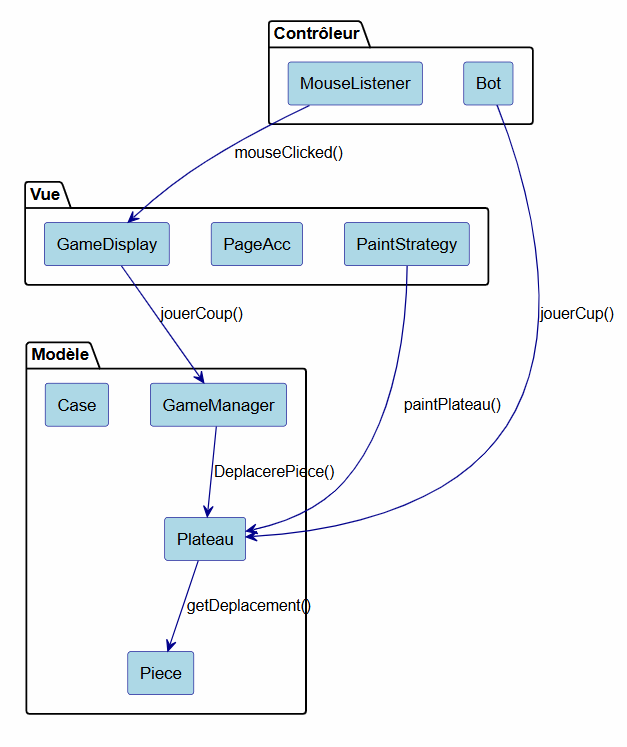
\includegraphics[width=12cm, height=12cm]{images/diagrammeMVC.png}
\caption{Architecture MVC du projet }
\label{fig:accueil1}
\end{figure}

\subsection{Packages }
\paragraph{} Voici la structure complète des packages du projet :
\begin{itemize}
\item \texttt{config} : constantes globales comme la taille du plateau et des cases ;
\item \texttt{engine.map} : contient \texttt{Plateau}, \texttt{Case}, \texttt{CaseNormal}, \texttt{CaseMort}, \texttt{Couleur}, \texttt{TypeCaseNormale} ;
\item \texttt{engine.mobile} : contient la classe abstraite \texttt{Piece} et ses sous-classes \texttt{General}, \texttt{Conseillere}, \texttt{Elephant}, \texttt{Chevalier}, \texttt{Char}, \texttt{Canon}, \texttt{Soldat} ;
\item \texttt{engine.process} : contient \texttt{GameManager}, \texttt{Bot}, \texttt{Coup}, \texttt{Niveau} ;
\item \texttt{gui} : contient \texttt{MainGUI}, \texttt{PageAcc}, \texttt{GameDisplay}, \texttt{PaintStrategy} ;
\item \texttt{log} : configuration des logs avec Log4j ;
\item \texttt{junit} : tests unitaires avec JUnit.
\end{itemize}
%\begin{figure}
%\centering
%\includegraphics[width=3.5cm, height=2cm]{images/architecture.png}
%\caption{Architecture MVC du projet}
%\label{fig:architecture}
%\end{figure}


\subsection{Classes de données}
\begin{figure}[H]
\centering
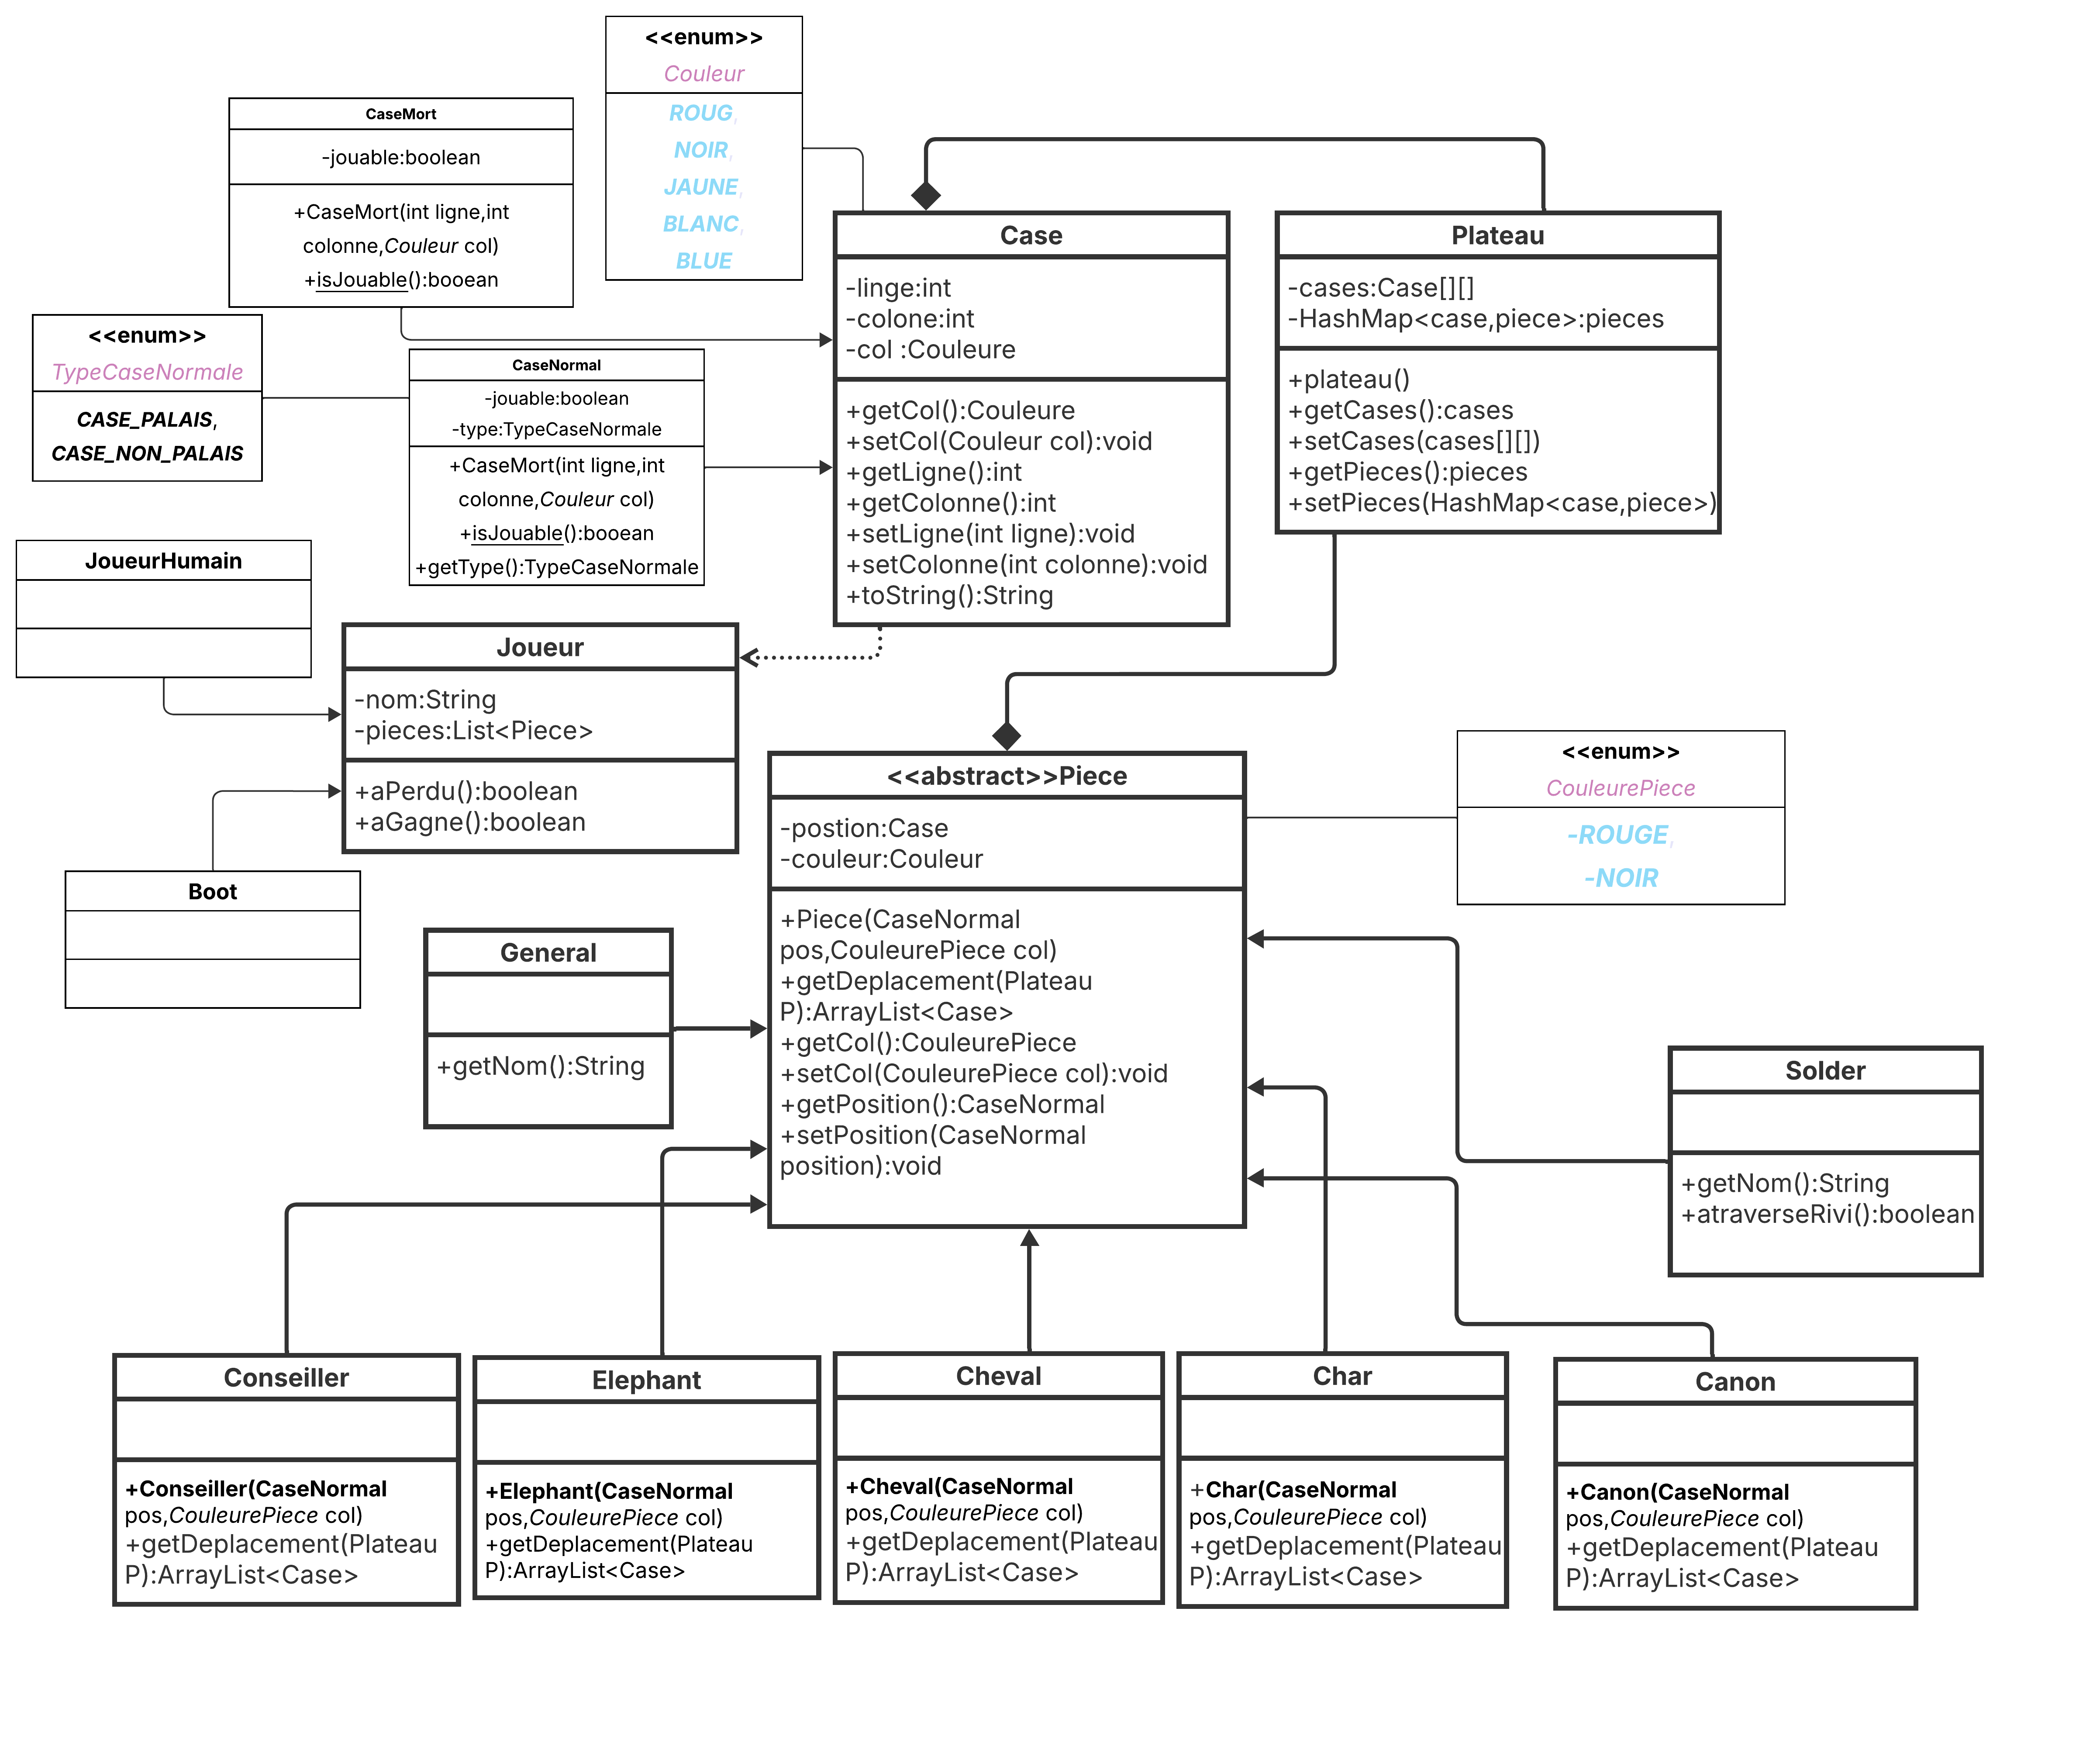
\includegraphics[width=16cm, height=14cm]{images/diagrammeclasses.png}
\caption{Diagramme de classes }
\label{fig:accueil2}
\end{figure} 


\subsubsection{La classe Plateau}
\paragraph{} La classe Plateau est au cœur du projet. Elle représente l'état complet du jeu à tout moment. Elle contient :
\begin{itemize}
\item un tableau \texttt{Case[11][11]} qui représente la grille du plateau ;
\item une \texttt{HashMap<Case, Piece>} qui associe chaque case occupée à sa pièce ;
\item la couleur du joueur dont c'est le tour (\texttt{CouleurePiece}) ;
\item deux listes pour stocker les pièces capturées (une par couleur).
\end{itemize}
\subsubsection{Initialisation du plateau}
\paragraph{} Au démarrage, les cases neutres (colonnes 3 et 7) et la rivière (ligne 5) sont initialisées comme des \texttt{CaseMort}. Les cases du palais sont de type \texttt{CASE\_PALAIS}.
\subsubsection{Méthodes principales}
\paragraph{} Les méthodes les plus importantes de \texttt{Plateau} sont :
\begin{itemize}
\item \texttt{coupValide(depart, arrivee)} : simule un coup et vérifie que le Général n'est pas en échec et qu'il n'y a pas de face à face après le coup ;
\item \texttt{estMenacer(case, couleur)} : vérifie si une case est attaquée par une couleur donnée ;
\item \texttt{EnEchec(joueur)} : dit si un joueur est actuellement en échec ;
\item \texttt{EnEchecEtMat(joueur)} : vérifie si un joueur n'a plus aucun coup légal ;
\item \texttt{RoiFacAfac()} : détecte si les deux Généraux sont sur la même colonne sans pièce entre eux.
\end{itemize}
\subsubsection{La hiérarchie des pièces}
\paragraph{} La classe abstraite \texttt{Piece} définit la méthode \texttt{getDeplacement(Plateau)} que chaque sous-classe redéfinit selon ses propres règles. Par exemple, le \texttt{Canon} parcourt les cases horizontalement et verticalement en ignorant les colonnes neutres, et cherche un écran avant de pouvoir capturer.



\subsection{IHM Graphique}
\paragraph{} L'interface graphique est faite avec \textbf{Java Swing} et est composée de trois classes principales :
\begin{itemize}
\item \texttt{PageAcc} : la page d'accueil avec un fond d'image, le titre du jeu, et les boutons pour choisir le mode de jeu. En mode VS BOT, un second dialogue apparaît pour choisir la difficulté ;
\item \texttt{GameDisplay} : le panneau principal pendant la partie. Il contient le plateau au centre, les zones de captures en haut et en bas, et un panneau à droite avec l'historique des coups et le bouton menu ;
\item \texttt{PaintStrategy} : s'occupe uniquement du rendu graphique — dessine les cases, les pièces (images PNG) et les surbrillances des coups légaux.
\end{itemize}
\subsection{Conception des traitements (processus)}

\subsubsection{Diagramme de sequence}
\begin{figure}[H]
\centering
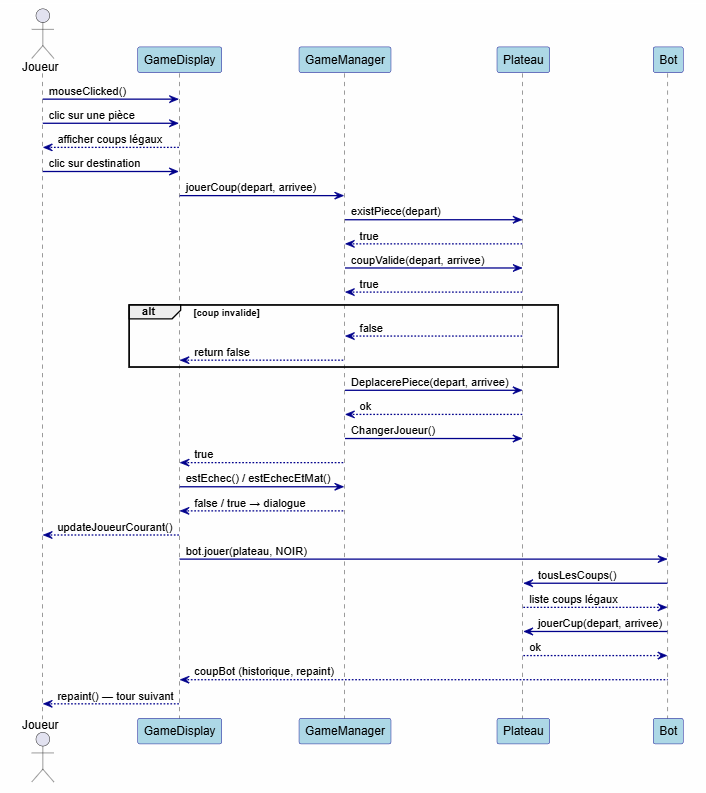
\includegraphics[width=15cm, height=15cm]{images/diagrammesequence.png}
\label{fig:accueil3}
\end{figure}

\subsubsection{Les niveaux du bot}
\paragraph{} Le bot dispose de trois niveaux définis dans l'énumération \texttt{Niveau} :
\begin{itemize}
\item \textbf{Facile} : le bot choisit un coup au hasard parmi tous ses coups légaux ;
\item \textbf{Moyen} : le bot essaie de capturer la pièce adverse la plus précieuse, en vérifiant d'abord que la case d'arrivée n'est pas dangereuse pour lui ;
\item \textbf{Difficile} : le bot calcule un score pour chaque coup possible. Ce score prend en compte la valeur de la pièce capturée, le danger pour ses propres pièces, la mise en échec de l'adversaire et la sécurité de son Général.
\end{itemize}
\paragraph{} Le tableau \ref{tab:valeurs} montre les valeurs utilisées par le bot pour évaluer les pièces.

\begin{table}[H]
\centering
\begin{tabular} {|p{3.5cm}|p{2cm}|}
\hline
\textbf{Pièce} & \textbf{Valeur} \\
\hline
Général & 100 \\
\hline
Chariot & 9 \\
\hline
Canon & 5 \\
\hline
Chevalier & 4 \\
\hline
Éléphant & 3 \\
\hline
Conseillère & 2 \\
\hline
Soldat & 1 \\
\hline
\end{tabular}
\caption{Valeurs des pièces utilisées par le bot}
\label{tab:valeurs}
\end{table}

\subsubsection{Validation des coups}
\paragraph{} Dans l'algorithme1, on décrit comment un coup est validé avant d'être joué.

\begin{algorithm}[H]
\caption{Validation d'un coup avant de jouer}
\label{algo:valide}
\begin{algorithmic}
\REQUIRE Départ $d$, Arrivée $a$, Plateau $P$
\ENSURE Vrai si le coup est légal, Faux sinon
\IF{$a \notin$ getDeplacement($d$, $P$)}
    \RETURN Faux
\ENDIF
\STATE Simuler : déplacer la pièce de $d$ vers $a$
\IF{le Général du joueur courant est menacé}
    \RETURN Faux
\ENDIF
\IF{les deux Généraux sont face à face}
    \RETURN Faux
\ENDIF
\STATE Annuler la simulation
\RETURN Vrai
\end{algorithmic}
\end{algorithm}
%%% Une autre façon pour écrire un algorithme %%%
%\begin{algorithm}[H]
 %\KwData{this text}
 %\KwResult{how to write algorithm with \LaTeX2e }
 %initialization\;
 %\While{not at end of this document}{
  %read current\;
  %\eIf{understand}{
   %go to next section\;
   %current section becomes this one\;
   %}{
   %go back to the beginning of current section\;
  %}
 %}
 %\caption{How to write algorithms}
%\end{algorithm}

\subsubsection{Tests unitaires}
\paragraph{} Les tests unitaires sont dans la classe \texttt{PlateauTest} et utilisent JUnit. On a testé les cas suivants :
\begin{itemize}
\item Le plateau et les pièces sont bien initialisés au démarrage ;
\item Le premier joueur est bien ROUGE ;
\item Le changement de joueur fonctionne correctement après un coup ;
\item La détection de présence ou d'absence de pièce sur une case ;
\item Un coup valide est bien accepté, un coup invalide est bien refusé ;
\item La détection des cases de bordure ;
\item Les deux Généraux sont bien présents sur le plateau ;
\item Aucun joueur n'est en échec au début de la partie ;
\item Une capture est bien enregistrée dans la liste correspondante ;
\item Les Généraux ne sont pas face à face en position initiale.
\end{itemize}


\newpage
\section{Manuel utilisateur}
\label{sec:manuel}
\subsection{Prérequis}
Pour faire tourner CHESS, il faut :
\begin{itemize}
\item Java JDK 1.8 ou supérieur installé sur la machine ;
\item Eclipse IDE ;
\item La librairie \texttt{log4j-1.2.17.jar} fournie par l'enseignant.
\end{itemize}
\subsection{Importer et configurer le projet sous Eclipse}
\paragraph{Importer le projet :}
\begin{enumerate}
\item Ouvrir Eclipse
\item Aller dans \texttt{File} $\rightarrow$ \texttt{Import}
\item Choisir \texttt{Existing Projects into Workspace}
\item Sélectionner le dossier du projet et valider
\end{enumerate}
\paragraph{Ajouter la librairie Log4j :}
\begin{enumerate}
\item Clic droit sur le projet $\rightarrow$ \texttt{Properties}
\item Aller dans \texttt{Java Build Path} $\rightarrow$ \texttt{Libraries}
\item Cliquer sur \texttt{Add External JARs} et sélectionner \texttt{log4j-1.2.17.jar}
\item Valider avec \texttt{Apply and Close}
\end{enumerate}
\paragraph{Lancer le jeu :}
\begin{enumerate}
\item Aller dans le package \texttt{gui}
\item Faire un clic droit sur \texttt{MainGUI.java}
\item Choisir \texttt{Run As} $\rightarrow$ \texttt{Java Application}
\end{enumerate}
\subsection{Utilisation du jeu}
\paragraph{Page d'accueil} Au lancement, on arrive sur la page d'accueil avec deux boutons :
\begin{itemize}
\item \textbf{VS BOT} : jouer contre l'ordinateur. Un menu s'ouvre pour choisir la difficulté (Facile, Moyen ou Difficile) ;
\item \textbf{VS HUMAIN} : jouer à deux joueurs sur la même machine, chacun son tour.
\end{itemize}
\begin{figure}[H]
\centering
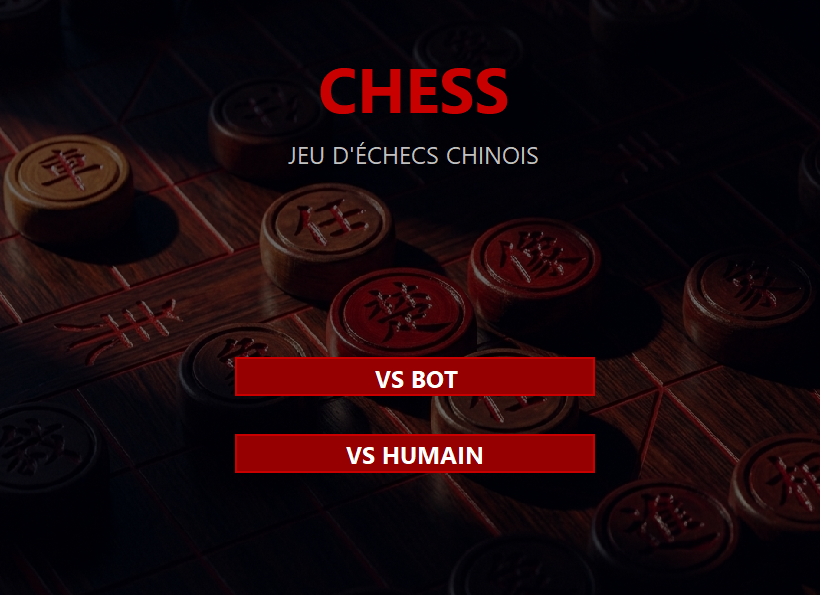
\includegraphics[width=10cm, height=7cm]{images/acceuil.png}
\caption{Page d'accueil de CHESS}
\label{fig:accueil}
\end{figure}
\paragraph{Pendant une partie}
\begin{itemize}
\item Pour jouer, on clique d'abord sur une de nos pièces — les cases où elle peut aller s'affichent en surbrillance ;
\item On clique ensuite sur une case en surbrillance pour effectuer le déplacement ;
\item Si on clique ailleurs, la sélection est annulée ;
\item Les pièces capturées apparaissent dans les panneaux en haut (noires capturées) et en bas (rouges capturées) du plateau ;
\item L'historique des coups joués s'affiche dans le panneau à droite avec la couleur du joueur correspondant ;
\item L'indicateur en bas à droite montre en permanence à qui c'est le tour (RED ou BLACK).
\end{itemize}
\begin{figure}[H]
\centering
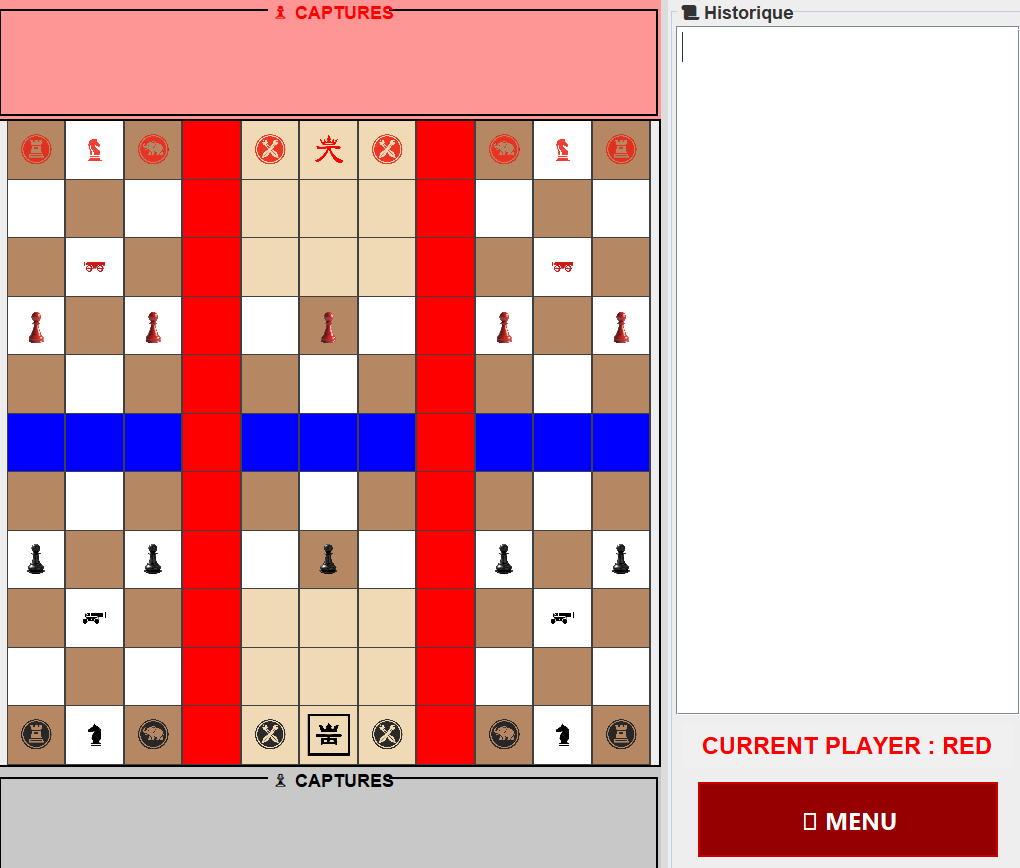
\includegraphics[width=13cm, height=9cm]{images/plateau.png}
\caption{Plateau de jeu pendant une partie}
\label{fig:partie}
\end{figure}
\paragraph{Menu en cours de partie} Le bouton \textbf{MENU} ouvre un dialogue avec trois options :
\begin{itemize}
\item \textbf{Reprendre} : ferme le menu et continue la partie ;
\item \textbf{Nouvelle Partie} : remet le plateau à zéro ;
\item \textbf{Quitter} : retourne à la page d'accueil.
\end{itemize}
\begin{figure}[H]
\centering
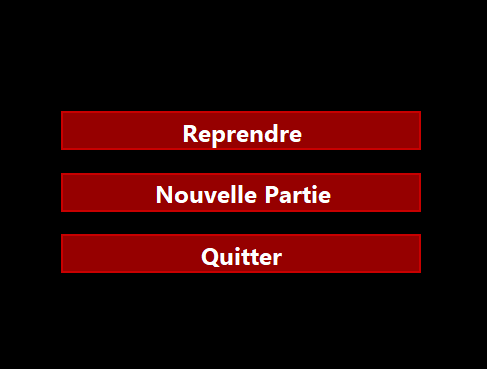
\includegraphics[width=6cm, height=5cm]{images/menu.png}
\caption{Menu en cours de partie}
\label{fig:menu}
\end{figure}
\paragraph{Fin de partie} Quand un joueur est en échec, une boîte de dialogue l'avertit. Quand il est en échec et mat, la partie se termine automatiquement et on ne peut plus jouer. 

\newpage
\section{Déroulement du projet}
\subsection{Réalisation du projet par étapes}
On a découpé le projet en plusieurs étapes successives :
\begin{enumerate}
\item Lecture et analyse des spécifications, puis conception de l'architecture MVC et des diagrammes UML ;
\item Mise en place des classes de base : plateau, cases, hiérarchie des pièces ;
\item Implémentation des règles de déplacement de chaque pièce, en gérant les colonnes neutres ;
\item Développement de la logique de validation des coups, de la détection d'échec et de la règle face à face ;
\item Développement de l'interface graphique avec Java Swing ;
\item Implémentation du bot et de ses trois niveaux de difficulté ;
\item Mise en place du système de logs avec Log4j ;
\item Écriture des tests unitaires JUnit ;
\item Rédaction du rapport.
\end{enumerate}
\subsection{Répartition des tâches, communication et intégration}
\paragraph{KETFI Ramdane}
S'est occupé du moteur de jeu et des classes de données : le plateau, la hiérarchie des pièces, la validation des coups, la détection d'échec, l'échec et mat, et la règle du face à face.
\paragraph{SOW Mamadou Saliou}
S'est occupé de l'interface graphique : la page d'accueil, le plateau de jeu, l'affichage des pièces capturées et l'historique des coups.
\paragraph{DJERMOUNE Thanina}
S'est occupée du bot et de ses trois niveaux de difficulté, ainsi que de la rédaction du rapport.
\paragraph{Communication et intégration}
Pour communiquer et partager notre travail, on a utilisé un groupe WhatsApp où on s'envoyait régulièrement les fichiers du projet sous forme de zip. On a aussi utilisé GitHub pour centraliser le code et éviter les conflits entre nos versions. Cela nous permettait de toujours avoir la dernière version du code et d'avancer ensemble malgré nos emplois du temps différents.
\paragraph{Difficultés rencontrées}
Au cours du projet, nous avons fait face à deux types de difficultés :
\begin{itemize}
\item \textbf{Difficultés organisationnelles :} Des divergences d'opinions ont parfois émergé au sein de l'équipe concernant certains choix techniques et de conception. Cependant, nous avons toujours privilégié le dialogue et la recherche d'un consensus, ce qui nous a permis de maintenir une cohésion solide tout au long du projet.
\item \textbf{Difficultés techniques :} La modélisation initiale du plateau et la hiérarchie des classes, notamment la gestion des colonnes neutres et de la rivière, ont nécessité une réflexion approfondie sur l'architecture du projet. L'intégration du bot au moteur de jeu a également été complexe, en particulier la conception d'un algorithme d'évaluation cohérent pour les niveaux Moyen et Difficile. Ces défis nous ont poussés à revoir certaines de nos décisions de conception, et nous en sommes sortis avec une meilleure compréhension du développement logiciel en équipe.
\end{itemize}
\newpage
\section{Conclusion et perspectives}
\subsection{Résumé du travail réalisé}
Au final, on a réussi à développer un jeu d'échecs chinois fonctionnel avec les éléments suivants :
\begin{itemize}
\item Un plateau 11×11 avec colonnes neutres et rivière, qui respecte toutes les spécifications ;
\item Les règles de déplacement de toutes les pièces, avec la gestion correcte des colonnes neutres ;
\item Un moteur de jeu qui valide chaque coup, détecte l'échec, l'échec et mat, et la règle du face à face ;
\item Un mode deux joueurs et un mode contre le bot avec trois niveaux de difficulté ;
\item Une interface graphique Swing avec historique des coups et affichage des captures ;
\item Un système de logs avec Log4j et des tests unitaires avec JUnit.
\end{itemize}
Ce projet nous a vraiment aidés à comprendre l'importance de bien séparer les responsabilités dans un logiciel, et à travailler en équipe sur un projet Java de taille réelle.
\subsection{Améliorations possibles du projet}
Si on avait eu plus de temps, on aurait voulu :
\begin{itemize}
\item Améliorer le bot avec un algorithme Minimax et l'élagage alpha-bêta pour le rendre plus fort ;
\item Ajouter une fonctionnalité de sauvegarde et de chargement de partie ;
\item Ajouter la rotation automatique du plateau en mode deux joueurs pour que chaque joueur voie son côté ;
\item Ajouter des animations pour les déplacements de pièces ;
\item Permettre de jouer en réseau contre un autre joueur.
\end{itemize}

\newpage
%Références bibliographiques du document
\bibliographystyle{alpha}
\bibliography{bibliographies}
\nocite{*}

\end{document}
